\documentclass{beamer}
\beamerdefaultoverlayspecification{<+->}
%
% Choose how your presentation looks.
%
% For more themes, color themes and font themes, see:
% http://deic.uab.es/~iblanes/beamer_gallery/index_by_theme.html
%
\mode<presentation>
{
  \usetheme{default}      % or try Darmstadt, Madrid, Warsaw, ...
  \usecolortheme{default} % or try albatross, beaver, crane, ...
  \usefonttheme{default}  % or try serif, structurebold, ...
  \setbeamertemplate{navigation symbols}{}
  \setbeamertemplate{caption}[numbered]
  \setbeamertemplate{footline}[frame number]
} 

\usepackage[english]{babel}
\usepackage[utf8]{inputenc}
\usepackage[T1]{fontenc}
\usepackage{graphicx}
\graphicspath{ {./images/} }
\usepackage{hyperref}
\usepackage{pgfplots}
\pgfplotsset{compat=1.7}

\hypersetup{
    colorlinks=true,
    linkcolor=blue,
    filecolor=magenta,      
    urlcolor=cyan,
    bookmarks=true,
    pdfpagemode=FullScreen,
    }

\title{Econ 200 Section AJ}
\author{Lukas Hager \\ \href{mailto:lghhager@uw.edu}{lghhager@uw.edu}}
\institute{Office Hours: Monday 8-9, Thursday 3:30-4:30}
\date{January 29, 2021}

\begin{document}

\begin{frame}
  \titlepage
\end{frame}

% Uncomment these lines for an automatically generated outline.
%\begin{frame}{Outline}
%  \tableofcontents
%\end{frame}

\begin{frame}{Your Questions}
    Do you have questions about what you've read in the text or heard in lecture?
\end{frame}

\begin{frame}{Writing Assignments}
    \begin{itemize}
        \item Generally pretty decent
        \item Signaling
        \item Housing supply
        \item Don't force a story
    \end{itemize}
\end{frame}

\begin{frame}{Concepts}
    \begin{itemize}
        \item Consumer Surplus
            \begin{itemize}
                \item Intuitively: the difference between your marginal benefit and the price of an item
                \item Graphically: the triangle between the demand curve and price
            \end{itemize}
        \item Producer Surplus
            \begin{itemize}
                \item Intuitively: the difference between your marginal cost and the price of an item
                \item Graphically: the triangle between the supply curve and price
            \end{itemize}
    \end{itemize}
\end{frame}

\begin{frame}{Concepts}
    \begin{itemize}
        \item Deadweight Loss
        \begin{itemize}
            \item Lost gains from trade
            \item Indicator of inefficiency
            \item Equity vs efficiency tradeoff
        \end{itemize}
    \end{itemize}
\end{frame}

\begin{frame}{Price Ceilings and Floors}
    Draw a price ceiling at \$12. What is the amount of shortage at this price? Draw and calculate the deadweight loss.
    \begin{center}
        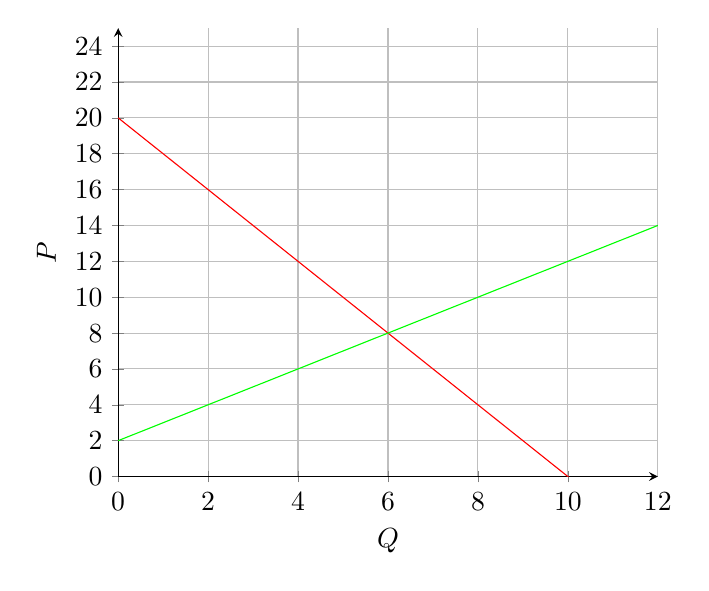
\begin{tikzpicture}
        \begin{axis}[
            axis lines = left,
            xlabel = $Q$,
            ylabel = $P$,
            ymax = 25,
            ymin = 0,
            xmax = 12,
            xmin = 0,
            scaled x ticks = false,
            ytick = {0,2,4,6,8,10,12,14,16,18,20,22,24},
            grid = both
        ]
        % \addplot [color=blue,fill=blue, 
        %                     fill opacity=0.05]
        %                     coordinates {
        %             (0, 10) 
        %             (0, 65/3)
        %             (70/3, 65/3)  };
        % \addplot [color=green,fill=green, 
        %         fill opacity=0.05]
        %         coordinates {
        %             (0, 65/3) 
        %             (70/3, 65/3)
        %             (0,45)};
        \addplot[
        color=red,
        domain=0:50,
        range = 0:50]{-2*x + 20};
        \addplot[
        color=green,
        domain=0:50,
        range = 0:50]{2+x};
        \end{axis}
        \end{tikzpicture}
    \end{center}
\end{frame}

\begin{frame}{Price Ceilings and Floors}
    \begin{center}
        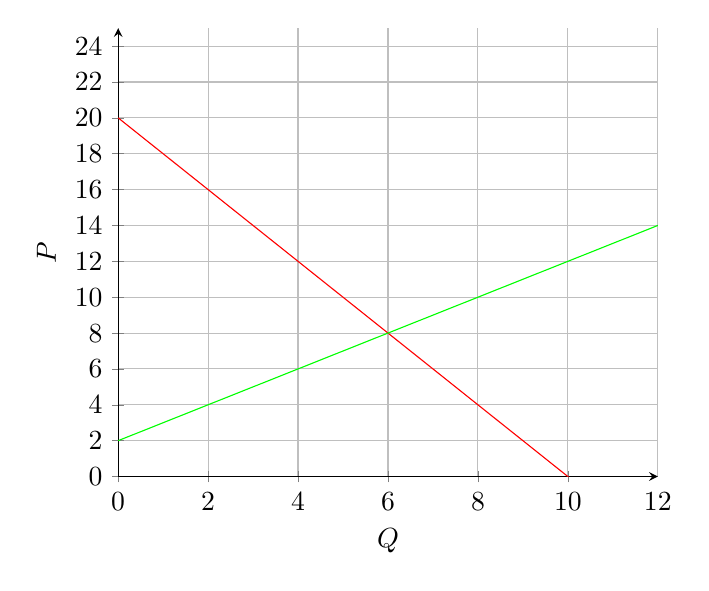
\begin{tikzpicture}
        \begin{axis}[
            axis lines = left,
            xlabel = $Q$,
            ylabel = $P$,
            ymax = 25,
            ymin = 0,
            xmax = 12,
            xmin = 0,
            scaled x ticks = false,
            ytick = {0,2,4,6,8,10,12,14,16,18,20,22,24},
            grid = both
        ]
        % \addplot [color=blue,fill=blue, 
        %                     fill opacity=0.05]
        %                     coordinates {
        %             (0, 10) 
        %             (0, 65/3)
        %             (70/3, 65/3)  };
        % \addplot [color=green,fill=green, 
        %         fill opacity=0.05]
        %         coordinates {
        %             (0, 65/3) 
        %             (70/3, 65/3)
        %             (0,45)};
        \addplot[
        color=red,
        domain=0:50,
        range = 0:50]{-2*x + 20};
        \addplot[
        color=green,
        domain=0:50,
        range = 0:50]{2+x};
        \end{axis}
        \end{tikzpicture}
    \end{center}
    Draw a price ceiling at \$4. What is the amount of shortage at this price? Draw and calculate the deadweight loss.
\end{frame}

\begin{frame}{Price Ceilings and Floors}
    \begin{center}
        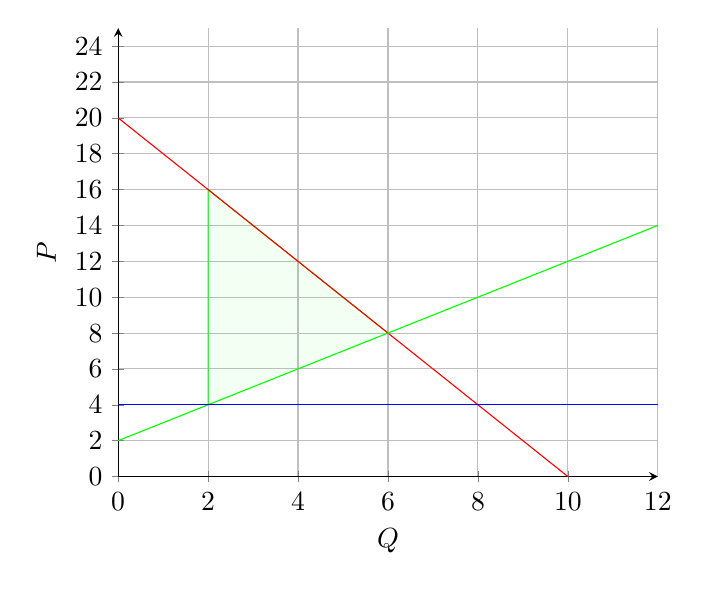
\begin{tikzpicture}
        \begin{axis}[
            axis lines = left,
            xlabel = $Q$,
            ylabel = $P$,
            ymax = 25,
            ymin = 0,
            xmax = 12,
            xmin = 0,
            scaled x ticks = false,
            ytick = {0,2,4,6,8,10,12,14,16,18,20,22,24},
            grid = both
        ]
        % \addplot [color=blue,fill=blue, 
        %                     fill opacity=0.05]
        %                     coordinates {
        %             (0, 10) 
        %             (0, 65/3)
        %             (70/3, 65/3)  };
        \addplot [color=green,fill=green, 
                fill opacity=0.05]
                coordinates {
                    (2, 4) 
                    (2, 16)
                    (6, 8)};
        \addplot[
        color=red,
        domain=0:50,
        range = 0:50]{-2*x + 20};
        \addplot[
        color=green,
        domain=0:50,
        range = 0:50]{2+x};
        \addplot[
        color=blue,
        domain=0:50,
        range = 0:50]{4};
        \end{axis}
        \end{tikzpicture}
    \end{center}
    Draw a price ceiling at \$4. What is the amount of shortage at this price? Draw and calculate the deadweight loss.
\end{frame}

\begin{frame}{Price Ceilings and Floors}
    \[
        \text{Shortage} = 8 - 2 = \boxed{6}
    \]
    \[\begin{split}
        \text{Deadweight Loss} &= \frac{bh}{2} \qquad \text{(triangle area)} \\
        &= \frac{(6-2)(\$16-\$4)}{2} \\
        &= \frac{4 \times \$12}{2} \\
        &= \boxed{\$24}
    \end{split}\]
\end{frame}

\begin{frame}[t]{Ironian(?) Brussel Sprouts}
    The Organization for the Promotion of Brussels Sprouts has convinced the government of Ironia to institute a price floor on the sale of brussel sprouts, at \$8 per bushel. Demand is given by $P = 9 - Q$ and supply by $P = 2Q$, where $Q$ is measured in thousands of bushels.
\end{frame}

\begin{frame}[t]{Ironian(?) Brussel Sprouts}
    The Organization for the Promotion of Brussels Sprouts has convinced the government of Ironia to institute a price floor on the sale of brussel sprouts, at \$8 per bushel. Demand is given by $P = 9 - Q$ and supply by $P = 2Q$, where $Q$ is measured in thousands of bushels.
    \begin{itemize}
        \item What will be the price and quantity of brussel sprouts sold at market equilibrium?
        \item What will be the price and quantity sold with the price floor?
        \item How big will be the excess supply of brussel sprouts produced with the price floor?
    \end{itemize}
\end{frame}

\begin{frame}[t]{Ironian(?) Brussel Sprouts}
   \textbf{ What will be the price and quantity of brussel sprouts sold at market equilibrium?}
\end{frame}

\begin{frame}[t]{Ironian(?) Brussel Sprouts}
    \textbf{What will be the price and quantity of brussel sprouts sold at market equilibrium?}
    \newline
    \newline Set $P_Q = P_D = P^*$:
    \[2Q^* = 9-Q^* \implies \boxed{Q^* = 3}\]
    Plug $Q^*$ into either equation to get $P^*$:
    \[P^* = 2Q^* \implies \boxed{P^* = \$6}\]
\end{frame}

\begin{frame}[t]{Ironian(?) Brussel Sprouts}
    \textbf{What will be the price and quantity sold with the price floor?}
\end{frame}

\begin{frame}[t]{Ironian(?) Brussel Sprouts}
    \textbf{What will be the price and quantity sold with the price floor?}
    \newline
    \newline Note that the price floor is higher than the equilibrium price -- thus, the floor will bind, and demand will constrain the market, so we use that condition:
    \[8 = 9 - Q_D \implies \boxed{Q_D = 1}\]
    The price is trivially $P^* = 8$ by the price floor (as it binds)
\end{frame}

\begin{frame}[t]{Ironian(?) Brussel Sprouts}
    \textbf{How big will be the excess supply of brussel sprouts produced with the price floor?}
\end{frame}

\begin{frame}[t]{Ironian(?) Brussel Sprouts}
    \textbf{How big will be the excess supply of brussel sprouts produced with the price floor?}
    \newline 
    \newline We have to compare the quantity demanded to the quantity supplied at the price floor. We calculated the quantity demanded in the previous part, and quantity supplied will be given by
    \[8 = 2Q \implies \boxed{Q_S = 4}\]
    So 4,000 bushels are supplied and 1,000 are demanded, so the surplus will be given by
    \[\text{Surplus} = 4-1 = 3\]
    Thus, the surplus is 3,000 bushels.
\end{frame}

\begin{frame}{Taxes}
    Suppose there is a \$1.50 per unit tax levied on sellers. The initial supply curve is given by $P=1+0.025Q$. After the tax, the supply curve is given by $P=2.5+0.025Q$.
    \begin{center}
        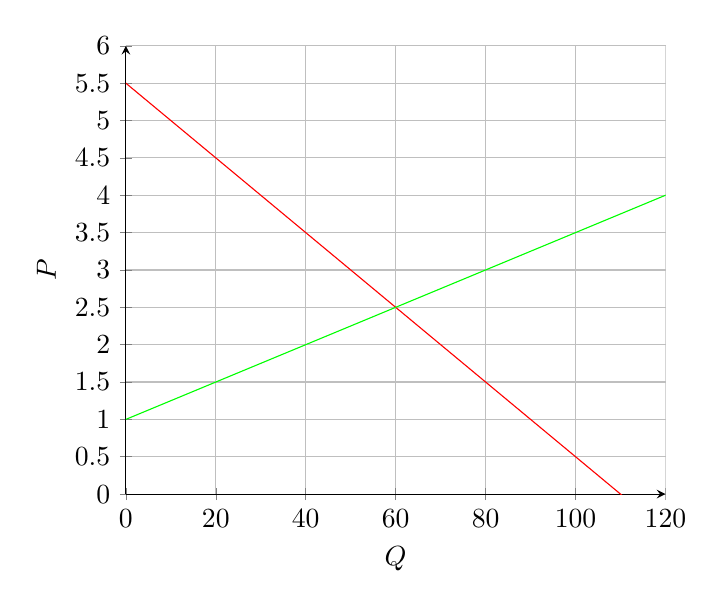
\begin{tikzpicture}
        \begin{axis}[
            axis lines = left,
            xlabel = $Q$,
            ylabel = $P$,
            ymax = 6,
            ymin = 0,
            xmax = 120,
            xmin = 0,
            scaled x ticks = false,
            ytick = {0,.5,1,1.5,2,2.5,3,3.5,4,4.5,5,5.5,6},
            grid = both
        ]
        % \addplot [color=blue,fill=blue, 
        %                     fill opacity=0.05]
        %                     coordinates {
        %             (0, 10) 
        %             (0, 65/3)
        %             (70/3, 65/3)  };
        % \addplot [color=green,fill=green, 
        %         fill opacity=0.05]
        %         coordinates {
        %             (0, 65/3) 
        %             (70/3, 65/3)
        %             (0,45)};
        \addplot[
        color=red,
        domain=0:200,
        range = 0:200]{-3*x/60 + 5.5};
        \addplot[
        color=green,
        domain=0:200,
        range = 0:200]{1+0.025*x};
        \end{axis}
        \end{tikzpicture}
    \end{center}
\end{frame}

\begin{frame}{Taxes}
    Draw the after-tax supply curve.
    \begin{center}
        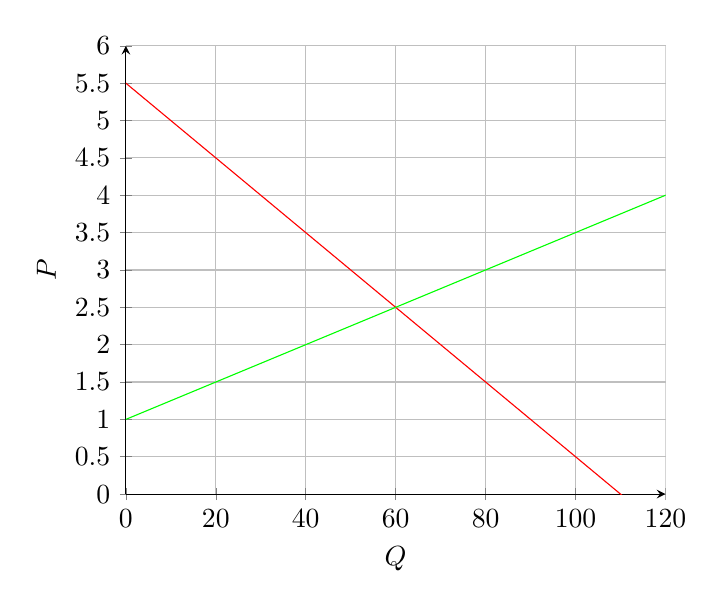
\begin{tikzpicture}
        \begin{axis}[
            axis lines = left,
            xlabel = $Q$,
            ylabel = $P$,
            ymax = 6,
            ymin = 0,
            xmax = 120,
            xmin = 0,
            scaled x ticks = false,
            ytick = {0,.5,1,1.5,2,2.5,3,3.5,4,4.5,5,5.5,6},
            grid = both
        ]
        % \addplot [color=blue,fill=blue, 
        %                     fill opacity=0.05]
        %                     coordinates {
        %             (0, 10) 
        %             (0, 65/3)
        %             (70/3, 65/3)  };
        % \addplot [color=green,fill=green, 
        %         fill opacity=0.05]
        %         coordinates {
        %             (0, 65/3) 
        %             (70/3, 65/3)
        %             (0,45)};
        \addplot[
        color=red,
        domain=0:200,
        range = 0:200]{-3*x/60 + 5.5};
        \addplot[
        color=green,
        domain=0:200,
        range = 0:200]{1+0.025*x};
        \end{axis}
        \end{tikzpicture}
    \end{center}
\end{frame}

\begin{frame}{Taxes}
    Draw the after-tax supply curve.
    \begin{center}
        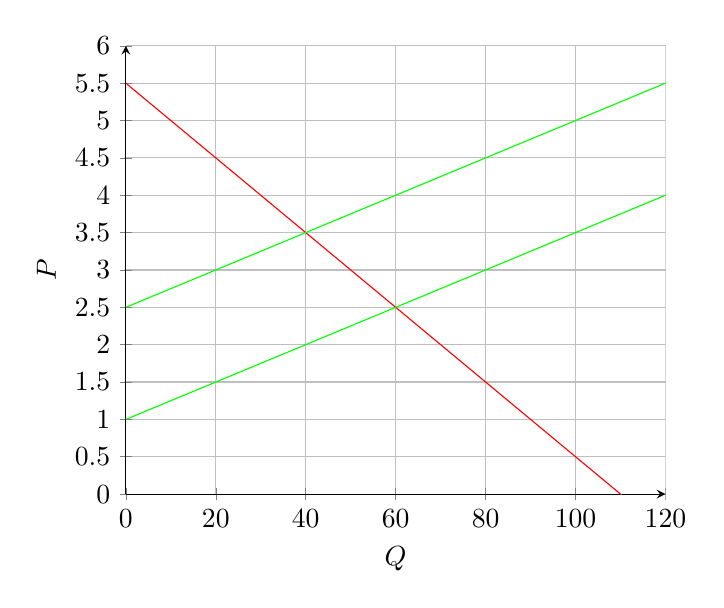
\begin{tikzpicture}
        \begin{axis}[
            axis lines = left,
            xlabel = $Q$,
            ylabel = $P$,
            ymax = 6,
            ymin = 0,
            xmax = 120,
            xmin = 0,
            scaled x ticks = false,
            ytick = {0,.5,1,1.5,2,2.5,3,3.5,4,4.5,5,5.5,6},
            grid = both
        ]
        % \addplot [color=blue,fill=blue, 
        %                     fill opacity=0.05]
        %                     coordinates {
        %             (0, 10) 
        %             (0, 65/3)
        %             (70/3, 65/3)  };
        % \addplot [color=green,fill=green, 
        %         fill opacity=0.05]
        %         coordinates {
        %             (0, 65/3) 
        %             (70/3, 65/3)
        %             (0,45)};
        \addplot[
        color=red,
        domain=0:200,
        range = 0:200]{-3*x/60 + 5.5};
        \addplot[
        color=green,
        domain=0:200,
        range = 0:200]{1+0.025*x};
        \addplot[
        color=green,
        domain=0:200,
        range = 0:200]{2.5+0.025*x};
        \end{axis}
        \end{tikzpicture}
    \end{center}
\end{frame}

\begin{frame}{Taxes}
    Plot the after-tax price paid by consumers and the after-tax price paid by sellers.
    \begin{center}
        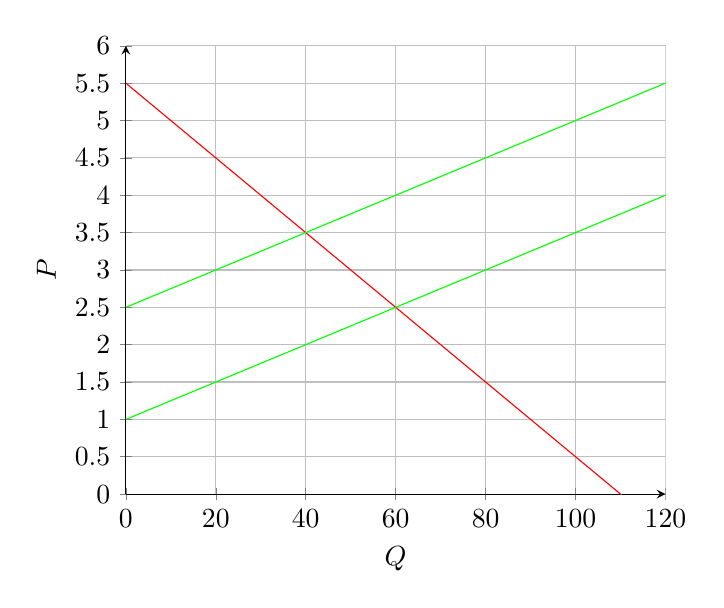
\begin{tikzpicture}
        \begin{axis}[
            axis lines = left,
            xlabel = $Q$,
            ylabel = $P$,
            ymax = 6,
            ymin = 0,
            xmax = 120,
            xmin = 0,
            scaled x ticks = false,
            ytick = {0,.5,1,1.5,2,2.5,3,3.5,4,4.5,5,5.5,6},
            grid = both
        ]
        % \addplot [color=blue,fill=blue, 
        %                     fill opacity=0.05]
        %                     coordinates {
        %             (0, 10) 
        %             (0, 65/3)
        %             (70/3, 65/3)  };
        % \addplot [color=green,fill=green, 
        %         fill opacity=0.05]
        %         coordinates {
        %             (0, 65/3) 
        %             (70/3, 65/3)
        %             (0,45)};
        \addplot[
        color=red,
        domain=0:200,
        range = 0:200]{-3*x/60 + 5.5};
        \addplot[
        color=green,
        domain=0:200,
        range = 0:200]{1+0.025*x};
        \addplot[
        color=green,
        domain=0:200,
        range = 0:200]{2.5+0.025*x};
        \end{axis}
        \end{tikzpicture}
    \end{center}
\end{frame}

\begin{frame}{Taxes}
    Plot the after-tax price paid by consumers and the after-tax price paid by sellers.
    \begin{center}
        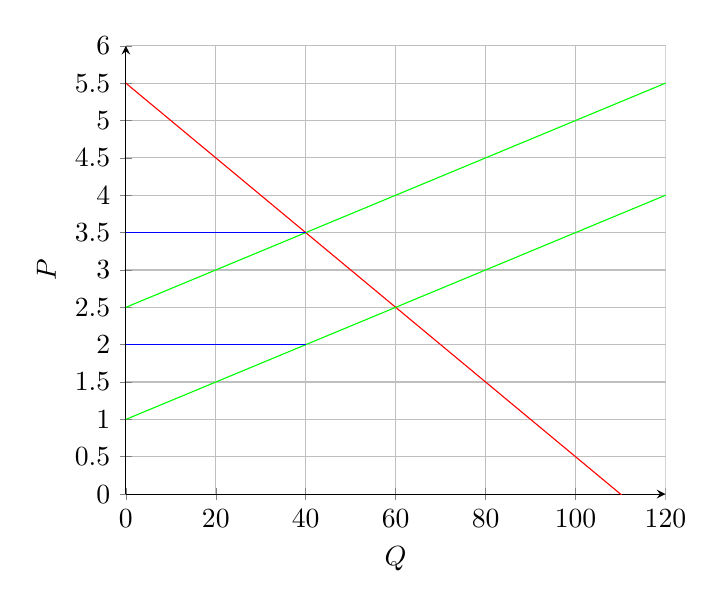
\begin{tikzpicture}
        \begin{axis}[
            axis lines = left,
            xlabel = $Q$,
            ylabel = $P$,
            ymax = 6,
            ymin = 0,
            xmax = 120,
            xmin = 0,
            scaled x ticks = false,
            ytick = {0,.5,1,1.5,2,2.5,3,3.5,4,4.5,5,5.5,6},
            grid = both
        ]
        % \addplot [color=blue,fill=blue, 
        %                     fill opacity=0.05]
        %                     coordinates {
        %             (0, 10) 
        %             (0, 65/3)
        %             (70/3, 65/3)  };
        % \addplot [color=green,fill=green, 
        %         fill opacity=0.05]
        %         coordinates {
        %             (0, 65/3) 
        %             (70/3, 65/3)
        %             (0,45)};
        \addplot[
        color=red,
        domain=0:200,
        range = 0:200]{-3*x/60 + 5.5};
        \addplot[
        color=green,
        domain=0:200,
        range = 0:200]{1+0.025*x};
        \addplot[
        color=green,
        domain=0:200,
        range = 0:200]{2.5+0.025*x};
        \addplot[
        color=blue,
        domain=0:40,
        range = 0:40]{2};
        \addplot[
        color=blue,
        domain=0:40,
        range = 0:40]{3.5};
        \end{axis}
        \end{tikzpicture}
    \end{center}
\end{frame}

\begin{frame}{Taxes}
    Draw consumer surplus, producer surplus, tax revenue, and deadweight loss after the tax.
    \begin{center}
        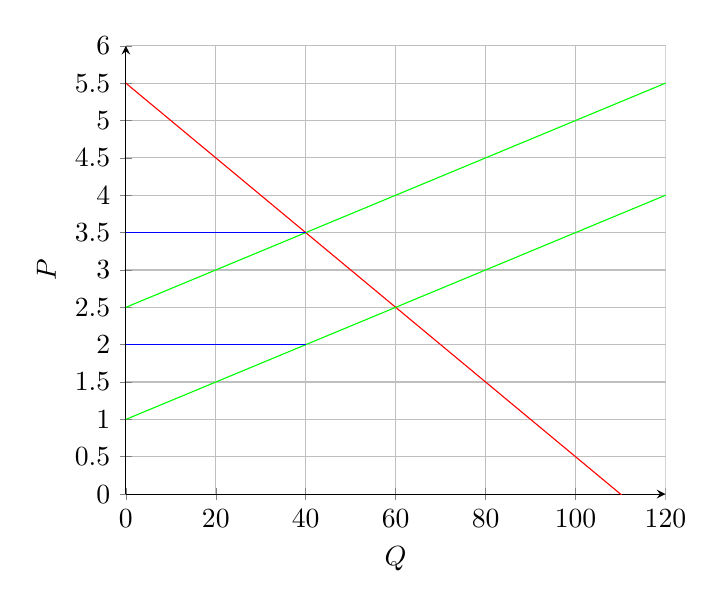
\begin{tikzpicture}
        \begin{axis}[
            axis lines = left,
            xlabel = $Q$,
            ylabel = $P$,
            ymax = 6,
            ymin = 0,
            xmax = 120,
            xmin = 0,
            scaled x ticks = false,
            ytick = {0,.5,1,1.5,2,2.5,3,3.5,4,4.5,5,5.5,6},
            grid = both
        ]
        % \addplot [color=blue,fill=blue, 
        %                     fill opacity=0.05]
        %                     coordinates {
        %             (0, 10) 
        %             (0, 65/3)
        %             (70/3, 65/3)  };
        % \addplot [color=green,fill=green, 
        %         fill opacity=0.05]
        %         coordinates {
        %             (0, 65/3) 
        %             (70/3, 65/3)
        %             (0,45)};
        \addplot[
        color=red,
        domain=0:200,
        range = 0:200]{-3*x/60 + 5.5};
        \addplot[
        color=green,
        domain=0:200,
        range = 0:200]{1+0.025*x};
        \addplot[
        color=green,
        domain=0:200,
        range = 0:200]{2.5+0.025*x};
        \addplot[
        color=blue,
        domain=0:40,
        range = 0:40]{2};
        \addplot[
        color=blue,
        domain=0:40,
        range = 0:40]{3.5};
        \end{axis}
        \end{tikzpicture}
    \end{center}
\end{frame}

\begin{frame}{Taxes}
    Draw consumer surplus, producer surplus, tax revenue, and deadweight loss after the tax.
    \begin{center}
        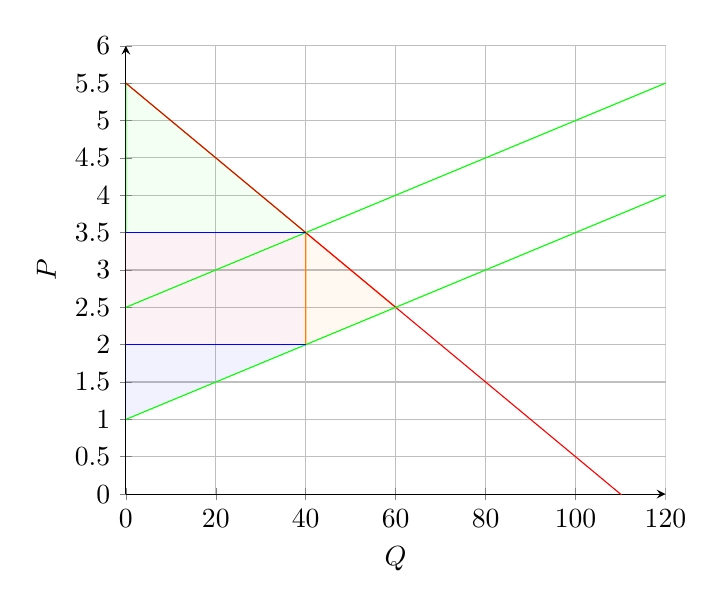
\begin{tikzpicture}
        \begin{axis}[
            axis lines = left,
            xlabel = $Q$,
            ylabel = $P$,
            ymax = 6,
            ymin = 0,
            xmax = 120,
            xmin = 0,
            scaled x ticks = false,
            ytick = {0,.5,1,1.5,2,2.5,3,3.5,4,4.5,5,5.5,6},
            grid = both
        ]
        \addplot [color=blue,fill=blue, 
                            fill opacity=0.05]
                            coordinates {
                    (0, 1) 
                    (0, 2)
                    (40, 2)  };
        \addplot [color=green,fill=green, 
                fill opacity=0.05]
                coordinates {
                    (0, 3.5) 
                    (0, 5.5)
                    (40,3.5)};
        \addplot [color=purple,fill=purple, 
                fill opacity=0.05]
                coordinates {
                    (0, 2) 
                    (0, 3.5)
                    (40, 3.5)
                    (40, 2)};
        \addplot [color=orange,fill=orange, 
                fill opacity=0.05]
                coordinates {
                    (40, 2) 
                    (40, 3.5)
                    (60, 2.5)};
        \addplot[
        color=red,
        domain=0:200,
        range = 0:200]{-3*x/60 + 5.5};
        \addplot[
        color=green,
        domain=0:200,
        range = 0:200]{1+0.025*x};
        \addplot[
        color=green,
        domain=0:200,
        range = 0:200]{2.5+0.025*x};
        \addplot[
        color=blue,
        domain=0:40,
        range = 0:40]{2};
        \addplot[
        color=blue,
        domain=0:40,
        range = 0:40]{3.5};
        \end{axis}
        \end{tikzpicture}
    \end{center}
\end{frame}

\begin{frame}[t]{Taxes}
    \textbf{Calculate deadweight loss.}
\end{frame}

\begin{frame}[t]{Taxes}
    \textbf{Calculate deadweight loss.}
    \newline
    \newline Deadweight loss is the wedge between supply and demand curves that has a vertex at the old equilibrium. We again use the area of a triangle to calculate:
    \[\begin{split}
        \text{Deadweight Loss} &= \frac{(\$3.5 - \$2)(60-40)}{2} \\
        &= \frac{\$1.5 \times 20}{2} \\
        &= \boxed{\$15}
    \end{split}\]
\end{frame}

\begin{frame}[t]{Taxes}
    \textbf{Calculate total surplus.}
\end{frame}

\begin{frame}[t]{Taxes}
    \textbf{Calculate total surplus.}
    \newline
    \newline Total surplus is the sum of consumer surplus, producer surplus, and tax revenue:
    \[\begin{split}
        \text{Total Surplus} &= CS + PS + TR \\
        &= \frac{(\$5.5-\$3.5)(40-0)}{2} \\
        &+ \frac{(\$2 - \$1)(40-0)}{2} \\
        &+ (\$3.5 - \$2)(40-0) \\
        &= \$40 + \$20 + \$60 \\
        &= \boxed{\$120}
    \end{split}\]
\end{frame}


% \begin{frame}{Elasticity}
%     \begin{itemize}
%         \item Price elasticity of demand describes the size of the change in the quantity demanded of a good or service when its price changes.
%         \begin{itemize}
%             \item When consumers’ buying decisions are highly influenced by price, we say that their demand is \textit{more elastic}.
%             \item When consumers are not very sensitive to price changes—that is, when they will buy approximately the same quantity, regardless of the price—we say that their demand is \textit{more inelastic}.
%         \end{itemize}
%         \item Elasticity calculation uses the midpoint formula:
%         \[\varepsilon = \frac{\frac{Q_{new} - Q_{old}}{\text{Average of $Q$}}}{\frac{P_{new} - P_{old}}{\text{Average of $P$}}} = \frac{Q_{new} - Q_{old}}{\frac{Q_{new} + Q_{old}}{2}} \frac{\frac{P_{new} + P_{old}}{2}}{P_{new} - P_{old}}\]
%         \item Price elasticity of demand is always negative (why?)
%     \end{itemize}
% \end{frame}

% \begin{frame}[t]{Determinants of PED}
%     What determines the price elasticity of demand?
% \end{frame}

% \begin{frame}[t]{Determinants of PED}
%     What determines the price elasticity of demand?
%     \begin{itemize}
%         \item Availability of substitutes
%         \item Degree of necessity
%         \item Cost relative to income
%         \item Adjustment time
%         \item Scope of the market
%     \end{itemize}
% \end{frame}

% \begin{frame}{Other Elasticities}
%     \begin{itemize}
%         \item Price elasticity of supply
%         \item Cross-price elasticity of demand
%         \item Income elasticity of demand
%     \end{itemize}
% \end{frame}

% \begin{frame}{Other Elasticities}
%     \begin{center}
%         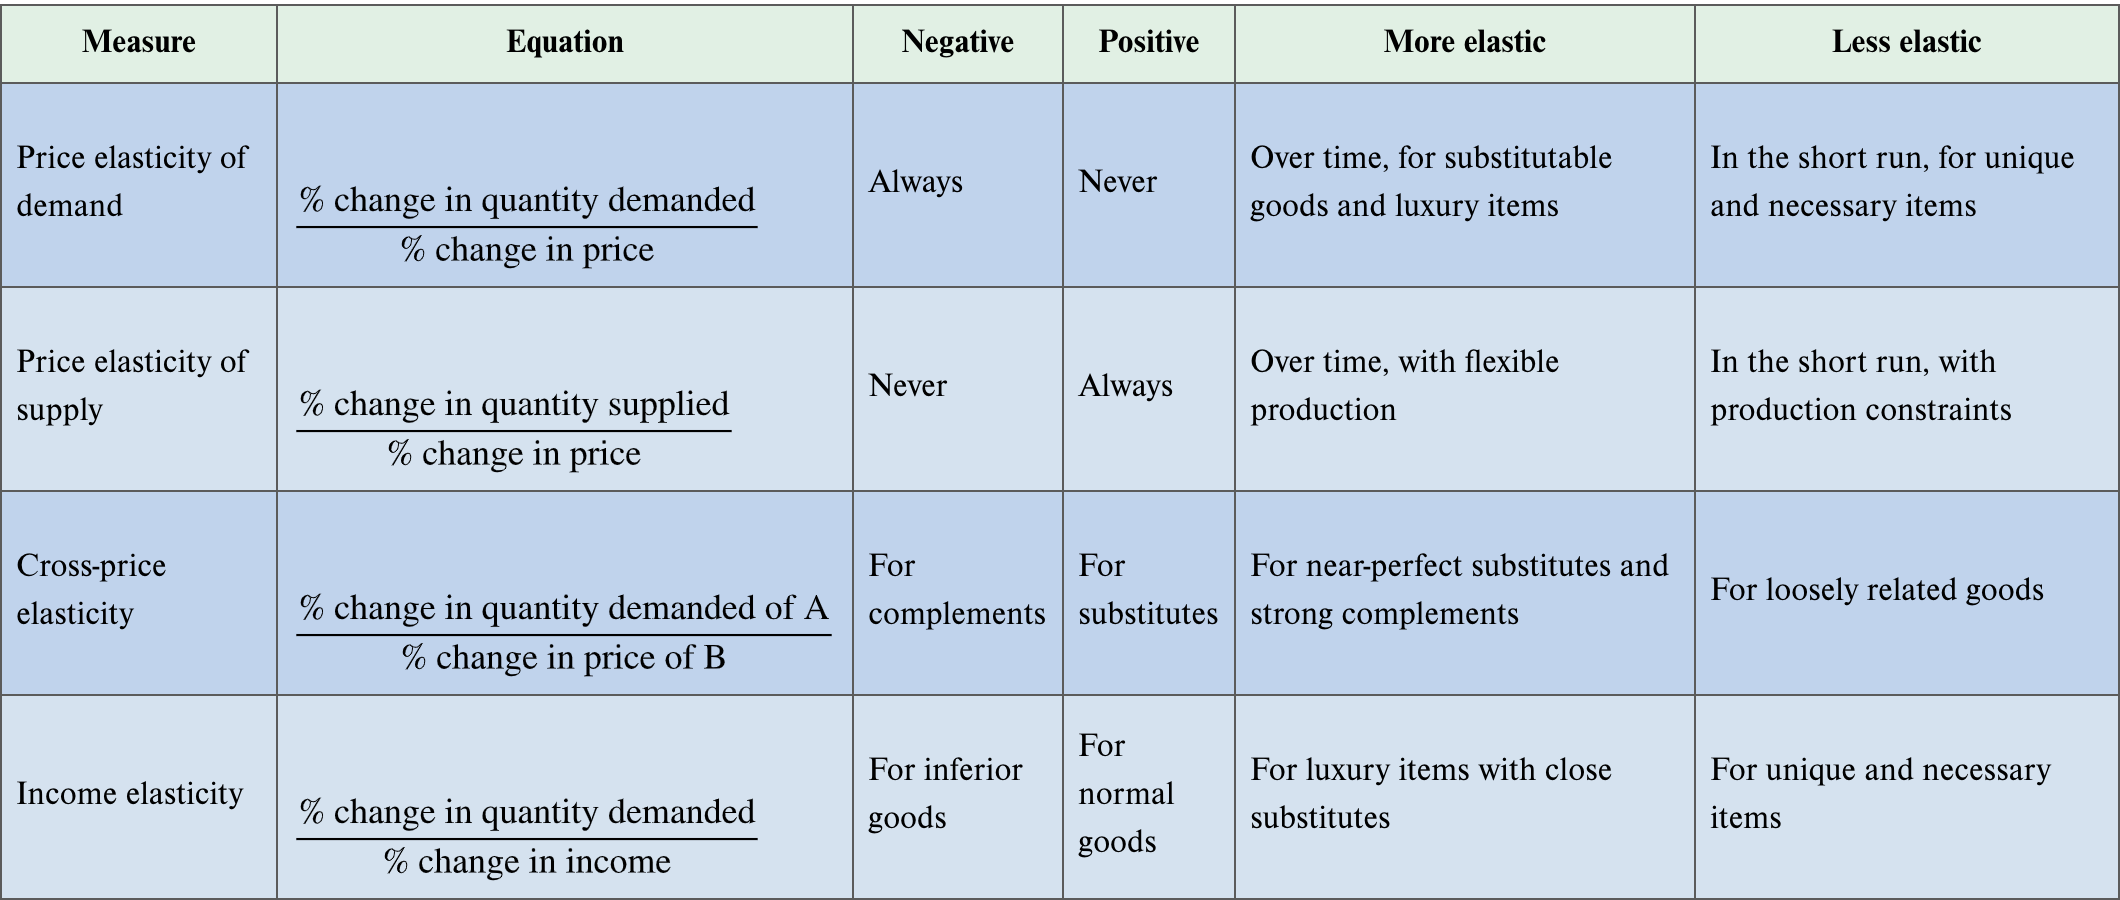
\includegraphics[scale=.3]{table}
%     \end{center}
% \end{frame}

% \begin{frame}{Surplus}
%     \begin{itemize}
%         \item Willingness to pay: the maximum price an agent is willing to pay for a good
%         \item Willingness to sell: the minimum price an agent is willing to sell a good for
%         % \item At prices above the maximum willingness to pay for consumers, the opportunity cost is greater than the benefits. At lower prices, the benefits outweigh the opportunity cost.
%         \item Surplus is a way of measuring who benefits from transactions and by how much. 
%         \begin{itemize}
%             \item The difference between willingness to pay/sell and the actual price.
%         \end{itemize}
%     \end{itemize}
% \end{frame}

% \begin{frame}{Elasticity Calculation}
%     \begin{tikzpicture}
%     \begin{axis}[
%         axis lines = left,
%         xmin=0, xmax=6,
%         ymin=0, ymax=25,
%         xlabel = {$Q$},
%         ylabel = {$P$},
%     ]
%     \addplot[thick] {-4*x + 20};
%     \node[label={0:{A (1,16)}},circle,fill,inner sep=2pt] at (axis cs:1, 16) {};
%     \node[label={0:{B (2,12)}},circle,fill,inner sep=2pt] at (axis cs:2, 12) {};
%     \end{axis}
%     \end{tikzpicture}
% \end{frame}

% \begin{frame}{Elasticity Calculation}
%     \[\begin{split}
%         \varepsilon &= \frac{\frac{Q_{new} - Q_{old}}{(Q_{old} + Q_{new}) / 2}}{\frac{P_{new} - P_{old}}{(P_{old} + P_{new}) / 2}} \\
%         &= \frac{\frac{2-1}{1.5}}{\frac{12-16}{14}} \\
%         &= -\frac{1}{1.5}\frac{14}{4}\\
%         &= -\frac{14}{6} \\
%         &\approx -2.33
%     \end{split}\]
% \end{frame}

% \begin{frame}{Perfectly Elastic Demand}
%     \begin{center}
%         \begin{tikzpicture}
%         \begin{axis}[
%         axis lines = left,
%         xlabel = $Q$,
%         ylabel = $P$,
%         xmin = -20,
%         ymin = -20,
%         xmax = 20,
%         ymax = 20,
%         yticklabels={,,},
%         xticklabels={,,},
%         ticks = none]
%         \end{axis}
%         \end{tikzpicture}
%     \end{center}
% \end{frame}

% \begin{frame}{Perfectly Inelastic Demand}
%     \begin{center}
%         \begin{tikzpicture}
%         \begin{axis}[
%         axis lines = left,
%         xlabel = $Q$,
%         ylabel = $P$,
%         xmin = -20,
%         ymin = -20,
%         xmax = 20,
%         ymax = 20,
%         yticklabels={,,},
%         xticklabels={,,},
%         ticks = none]
%         \end{axis}
%         \end{tikzpicture}
%     \end{center}
% \end{frame}

% \begin{frame}{Relatively More/Less Elastic Demand}
%     \begin{center}
%         \begin{tikzpicture}
%         \begin{axis}[
%         axis lines = left,
%         xlabel = $Q$,
%         ylabel = $P$,
%         xmin = 0,
%         ymin = 0,
%         xmax = 20,
%         ymax = 20,
%         yticklabels={,,},
%         xticklabels={,,},
%         ticks = none]
%         \addplot[thick][domain=0:20]{-1.3*x + 18};
%         \end{axis}
%         \end{tikzpicture}
%     \end{center}
% \end{frame}

% \begin{frame}[t]{Chocolate}
%     When the price of a bar of chocolate is \$1.00, the quantity demanded is 100,000 bars. When the price rises to \$1.50, the quantity demanded falls to 60,000 bars. Calculate the price elasticity of demand using the mid-point method.
% \end{frame}

% \begin{frame}{Chocolate}
%     \[\begin{split}
%         \varepsilon &= \frac{\frac{60,000 - 100,000}{80,000}}{\frac{1.50 - 1.00}{1.25}} \\
%         &= -\frac{.5}{\frac{.5}{1.25}} \\
%         &= \boxed{-1.25}
%     \end{split}\]
% \end{frame}

% \begin{frame}[t]{Chocolate}
%     When the price of a bar of chocolate is \$1.00, the quantity demanded is 100,000 bars. When the price rises to \$1.50, the quantity demanded falls to 60,000 bars. What is the price effect and quantity effect for this change? What happens to total revenue?
% \end{frame}

% \begin{frame}{Chocolate}
%     Price Effect:
%     \[\$0.50 \times 60,000 = \$30,000\]
%     Quantity Effect:
%     \[\$1 \times -40,000 = -\$40,000\]
%     Change in Total Revenue
%     \[\$30,000 - \$40,000 = -\$10,000\]
% \end{frame}

% \begin{frame}[t]{Used Cars}
%     If the price elasticity of demand for used cars priced between \$3,000 and \$5,000 is –1.2 (using the mid-point method), what will be the percent change in quantity demanded when the price of a used car falls from \$5,000 to \$3,000?
% \end{frame}

% \begin{frame}{Used Cars}
%     \[\begin{split}
%         -1.2 &= \frac{\text{\% Change in Quantity Demanded}}{\frac{3,000 - 5,000}{4,000}} \\
%         &=\frac{\text{\% Change in Quantity Demanded}}{\frac{-2,000}{4,000}} \\
%         &=\frac{\text{\% Change in Quantity Demanded}}{-.5} \\
%         \implies .6 &= \text{\% Change in Quantity Demanded} \\
%         \implies \boxed{60\%} &= \text{\% Change in Quantity Demanded} 
%     \end{split}\]
% \end{frame}

% \begin{frame}[t]{Short-Run Elasticity}
%     Which of the following has a more elastic demand in the short run?
% \end{frame}

% \begin{frame}[t]{Short-Run Elasticity}
%     Which of the following has a more elastic demand in the short run?
%     \begin{itemize}
%         \item Pomegranate juice or drinking water?
%         \item Cereal or Rice Krispies®?
%         \item Speedboats or gourmet chocolate?
%     \end{itemize}
% \end{frame}

% \begin{frame}[t]{Short-Run Elasticity}
%     Which of the following has a more elastic demand in the short run?
%     \begin{itemize}
%         \item \textbf{Pomegranate juice} or drinking water?
%         \item Cereal or \textbf{Rice Krispies®}?
%         \item \textbf{Speedboats} or gourmet chocolate?
%     \end{itemize}
% \end{frame}

% \begin{frame}{Surplus}
%     \begin{itemize}
%         \item What is marginal benefit?
%         \item Why is the demand curve referred to as the marginal benefit curve?
%         \item What is marginal cost?
%         \item Why is the supply curve referred to as the marginal cost curve?
%     \end{itemize}
% \end{frame}

% \begin{frame}[t]{Mona Lisa}
%     Suppose you are offered the chance to purchase the Mona Lisa for \$5 million, but you consider this painting to be (without any exaggeration) ``priceless". What is your consumer surplus?
% \end{frame}

% \begin{frame}[t]{Oranges}
%     Suppose the market for oranges looks like this:
%     \begin{center}
%         \begin{tikzpicture}
%         \begin{axis}[
%             axis lines = left,
%             xlabel = $Q$,
%             ylabel = $P$,
%             ymax = 50,
%             ymin = 0,
%             xmax = 50,
%             xmin = 0,
%             scaled x ticks = false,
%             ytick = {0,5,10,15,20,25,30,35,40,45,50}
%         ]
%         % \addplot [color=blue,fill=blue, 
%         %                     fill opacity=0.05]
%         %                     coordinates {
%         %             (0, 20) 
%         %             (0, 23)
%         %             (6, 20)  };
%         % \addplot [color=green,fill=green, 
%         %         fill opacity=0.05]
%         %         coordinates {
%         %             (0, 14) 
%         %             (0, 20)
%         %             (6,20)};
%         \addplot[
%         color=red,
%         domain=0:50,
%         range = 0:50]{-x + 45};
%         \addplot[
%         color=green,
%         domain=0:50,
%         range = 0:50]{10 + x/2};
%         % \addplot[
%         % color=black,
%         % domain=0:6,
%         % range = 0:6]{20};
%         \end{axis}
%         \end{tikzpicture}
%     \end{center}
% \end{frame}

% \begin{frame}[t]{Oranges}
%     A frost occurs, which destroys some of the orange crop. This shifts the supply curve left:
%     \begin{center}
%         \begin{tikzpicture}
%         \begin{axis}[
%             axis lines = left,
%             xlabel = $Q$,
%             ylabel = $P$,
%             ymax = 50,
%             ymin = 0,
%             xmax = 50,
%             xmin = 0,
%             scaled x ticks = false,
%             ytick = {0,5,10,15,20,25,30,35,40,45,50}
%         ]
%         % \addplot [color=blue,fill=blue, 
%         %                     fill opacity=0.05]
%         %                     coordinates {
%         %             (0, 20) 
%         %             (0, 23)
%         %             (6, 20)  };
%         % \addplot [color=green,fill=green, 
%         %         fill opacity=0.05]
%         %         coordinates {
%         %             (0, 14) 
%         %             (0, 20)
%         %             (6,20)};
%         \addplot[
%         color=red,
%         domain=0:50,
%         range = 0:50]{-x + 45};
%         \addplot[
%         color=green,
%         domain=0:50,
%         range = 0:50]{10 + x/2};
%         \addplot[
%         color=green,
%         domain=0:50,
%         range = 0:50]{20 + x/2};
%         \draw [->] (axis cs:10, 15) -- (axis cs:6, 23);
%         \draw [->] (axis cs:20, 20) -- (axis cs:16, 28);
%         \draw [->] (axis cs:30, 25) -- (axis cs:26, 33);
%         \draw [->] (axis cs:40, 30) -- (axis cs:36, 38);
%         % \addplot[
%         % color=black,
%         % domain=0:6,
%         % range = 0:6]{20};
%         \end{axis}
%         \end{tikzpicture}
%     \end{center}
% \end{frame}

% \begin{frame}[t]{Oranges}
%     Before the shift, the surplus allocations look like this:
%     \begin{center}
%         \begin{tikzpicture}
%         \begin{axis}[
%             axis lines = left,
%             xlabel = $Q$,
%             ylabel = $P$,
%             ymax = 50,
%             ymin = 0,
%             xmax = 50,
%             xmin = 0,
%             scaled x ticks = false,
%             ytick = {0,5,10,15,20,25,30,35,40,45,50}
%         ]
%         \addplot [color=blue,fill=blue, 
%                             fill opacity=0.05]
%                             coordinates {
%                     (0, 10) 
%                     (0, 65/3)
%                     (70/3, 65/3)  };
%         \addplot [color=green,fill=green, 
%                 fill opacity=0.05]
%                 coordinates {
%                     (0, 65/3) 
%                     (70/3, 65/3)
%                     (0,45)};
%         \addplot[
%         color=red,
%         domain=0:50,
%         range = 0:50]{-x + 45};
%         \addplot[
%         color=green,
%         domain=0:50,
%         range = 0:50]{10 + x/2};
%         \addplot[
%         color=green,
%         domain=0:50,
%         range = 0:50]{20 + x/2};
%         \addplot[
%         color=black,
%         domain=0:23.33,
%         range = 0:23.33]{65/3};
%         \end{axis}
%         \end{tikzpicture}
%     \end{center}
% \end{frame}

% \begin{frame}[t]{Oranges}
%     After the shift, the surplus allocations look like this:
%     \begin{center}
%         \begin{tikzpicture}
%         \begin{axis}[
%             axis lines = left,
%             xlabel = $Q$,
%             ylabel = $P$,
%             ymax = 50,
%             ymin = 0,
%             xmax = 50,
%             xmin = 0,
%             scaled x ticks = false,
%             ytick = {0,5,10,15,20,25,30,35,40,45,50}
%         ]
%         \addplot [color=blue,fill=blue, 
%                             fill opacity=0.05]
%                             coordinates {
%                     (0, 20) 
%                     (0, 85/3)
%                     (50/3, 85/3)  };
%         \addplot [color=green,fill=green, 
%                 fill opacity=0.05]
%                 coordinates {
%                     (0, 85/3) 
%                     (50/3, 85/3)
%                     (0,45)};
%         \addplot[
%         color=red,
%         domain=0:50,
%         range = 0:50]{-x + 45};
%         \addplot[
%         color=green,
%         domain=0:50,
%         range = 0:50]{10 + x/2};
%         \addplot[
%         color=green,
%         domain=0:50,
%         range = 0:50]{20 + x/2};
%         \addplot[
%         color=black,
%         domain=0:50/3,
%         range = 0:50/3]{85/3};
%         \end{axis}
%         \end{tikzpicture}
%     \end{center}
% \end{frame}

% \begin{frame}{Oranges}
%     Conclusions: the shift in supply decreases overall surplus, and also decreases the surplus of producers and consumers individually. This will not always be true, however!
% \end{frame}

% \begin{frame}{UW Football}
%     The demand for football tickets at the UW is $Q_D=80,000 - 500P$ and the supply is $QS=20,000$. Calculate the equilibrium price, quantity and Consumer/Producer Surplus.
% \end{frame}

% \begin{frame}{UW Football}
%     Recall that at equilibrium, $Q_S=Q_D=Q^*$. Thus, equilibrium quantity $Q^*$ must be 20,000. Substituting this into the demand condition yields
%     \[\begin{split}
%         &20,000 = 80,000 - 500P^* \\
%         \implies &-60,000 = -500P^* \\
%         \implies &\boxed{P^* = 120}
%     \end{split}\]
% \end{frame}

% \begin{frame}[t]{UW Football}
%     To calculate surplus, we visualize the market:
%     \begin{center}
%         \begin{tikzpicture}
%         \begin{axis}[
%             axis lines = left,
%             xlabel = $Q$,
%             ylabel = $P$,
%             ymax = 200,
%             ymin = 0,
%             xmax = 80000,
%             xmin = 0,
%             scaled x ticks = false,
%             ytick = {0,20,40,60,80,100,120,140,160,180,200}
%         ]
%         % \addplot [color=blue,fill=blue, 
%         %                     fill opacity=0.05]
%         %                     coordinates {
%         %             (0, 120) 
%         %             (0, 160)
%         %             (20000, 120)  };
%         % \addlegendentry[mark=*]{Consumer Surplus}
%         % \addplot [color=green,fill=green, 
%         %         fill opacity=0.05]
%         %         coordinates {
%         %             (0, 0) 
%         %             (0, 120)
%         %             (20000, 120)
%         %             (20000, 0)};
%         \addplot[
%         color=red,
%         domain=0:80000,
%         range = 0:80000]{-x/500 + 160};
%         \draw [color = green] (200,0) -- (200, 200);
%         \addplot[
%         color=black,
%         domain=0:20000,
%         range = 0:20000]{120};
%         \end{axis}
%         \end{tikzpicture}
%     \end{center}
    
% \end{frame}

% \begin{frame}[t]{UW Football}
%     To calculate surplus, we visualize the market:
%     \begin{center}
%         \begin{tikzpicture}
%         \begin{axis}[
%             axis lines = left,
%             xlabel = $Q$,
%             ylabel = $P$,
%             ymax = 200,
%             ymin = 0,
%             xmax = 80000,
%             xmin = 0,
%             scaled x ticks = false,
%             ytick = {0,20,40,60,80,100,120,140,160,180,200}
%         ]
%         \addplot [color=blue,fill=blue, 
%                             fill opacity=0.05]
%                             coordinates {
%                     (0, 120) 
%                     (0, 160)
%                     (20000, 120)  };
%         \addplot [color=green,fill=green, 
%                 fill opacity=0.05]
%                 coordinates {
%                     (0, 0) 
%                     (0, 120)
%                     (20000, 120)
%                     (20000, 0)};
%         \addplot[
%         color=red,
%         domain=0:80000,
%         range = 0:80000]{-x/500 + 160};
%         \draw [color = green] (200,0) -- (200, 200);
%         \addplot[
%         color=black,
%         domain=0:20000,
%         range = 0:20000]{120};
%         \end{axis}
%         \end{tikzpicture}
%     \end{center}
    
% \end{frame}

% \begin{frame}{UW Football}
%     Producer surplus is a rectangle:
%     \[PS = 20,000 \times \$120 = \$2,400,000\]
%     Consumer surplus is a triangle:
%     \[CS = \frac{1}{2}(\$40 \times 20,000) = \$400,000\]
% \end{frame}

% \begin{frame}{Arbitrary Market}
%     Given the following competitive market:
%     \[\begin{split}
%         Q_D&=46-2P \\
%         Q_S&=-14+P
%     \end{split}\]
%     Solve for the equilibrium and Consumer/Producer Surplus
% \end{frame}

% \begin{frame}[t]{Arbitrary Market}
%     \textbf{Equilibrium Calculation:}
% \end{frame}

% \begin{frame}[t]{Arbitrary Market}
%     \textbf{Equilibrium Calculation:}
%     \newline
%     \newline Set $Q_S = Q_D = Q^*$
%     \[\begin{split}
%         &46 - 2P = -14 + P^* \\
%         \implies &60 = 3P^* \\
%         \implies &\boxed{P^* = 20}
%     \end{split}\]
%     Substitution $P^*$ into either of the conditions to obtain $Q^*$:
%     \[\begin{split}
%         Q^* &= -14 + 20 \\
%         &= \boxed{6}
%     \end{split}\]
%     So the equilibrium is characterized by $(P^*, Q^*) = (20, 6)$
% \end{frame}

% \begin{frame}[t]{Arbitrary Market}
%     \textbf{Consumer/Producer Surplus:}
%     \begin{center}
%         \begin{tikzpicture}
%         \begin{axis}[
%             axis lines = left,
%             xlabel = $Q$,
%             ylabel = $P$,
%             ymax = 25,
%             ymin = 0,
%             xmax = 50,
%             xmin = 0,
%             scaled x ticks = false
%             % ytick = {0,20,40,60,80,100,120,140,160,180,200}
%         ]
%         \addplot [color=blue,fill=blue, 
%                             fill opacity=0.05]
%                             coordinates {
%                     (0, 20) 
%                     (0, 23)
%                     (6, 20)  };
%         \addplot [color=green,fill=green, 
%                 fill opacity=0.05]
%                 coordinates {
%                     (0, 14) 
%                     (0, 20)
%                     (6,20)};
%         \addplot[
%         color=red,
%         domain=0:50,
%         range = 0:50]{-x/2 + 23};
%         \addplot[
%         color=green,
%         domain=0:50,
%         range = 0:50]{14 + x};
%         \addplot[
%         color=black,
%         domain=0:6,
%         range = 0:6]{20};
%         \end{axis}
%         \end{tikzpicture}
%     \end{center}
% \end{frame}

% \begin{frame}[t]{Arbitrary Market}
%     \textbf{Consumer/Producer Surplus:}
%     \newline
%     \newline Consumer surplus will be a triangle, with legs from the y-axis at equilibrium price to the equilibrium and from the y-intercept of the demand curve to the equilibrium price:
%     \[CS = \frac{1}{2}((\$23-\$20) \times (6-0)) = \$9\]
%     Similarly, producer surplus will be a triangle, with legs from the y-axis at equilibrium price to the equilibrium and from the y-intercept of the supply curve to the equilibrium price:
%     \[PS = \frac{1}{2}((\$20-\$14) \times (6-0)) = \$18\]
% \end{frame}

% \begin{frame}{Midterm Question Spring 2018}
%     Suppose when the price of a cookie is \$2.50, the quantity demanded is 50, and when the price is \$1, the quantity demanded is 200.
%     \begin{itemize}
%         \item[a.] Using the midpoint method, calculate the price elasticity of demand. Although not asked in the original question–is this inelastic or elastic?
%         \item[b.] Calculate the change in total revenue due to the price change from \$2.50 to \$1. How much of that change is due to the price effect? How much is due to the quantity effect?
%         \item[c.] Suppose policy-makers think that Seattleites are eating too many cookies. Using the price elasticity you found in part (a), find how much the price of cookies will need to change (in percent) to make demand for cookies go down by 20\%. 
%         \item[d.] Which pair of goods is likely to have the largest positive cross-price elasticity? Underline your choice and explain your answer: Peanut butter and jelly, Butter and margarine, or Ramen noodles and a Rolex watch.
%     \end{itemize}
% \end{frame}

\end{document}
